\documentclass[a4paper, 12pt]{article}
\usepackage[utf8]{inputenc}
\usepackage[T1]{fontenc}
\usepackage[polish]{babel}
\usepackage{graphicx}
\usepackage{hyperref}
\usepackage{listings}
\usepackage{xcolor}
\setlength {\marginparwidth }{2cm}
\usepackage{todonotes}

\title{Dokumentacja aplikacji Unordered}
\author{Adam Dybcio\endline Łukasz Czapski\endline Igor Ciżewski\endline Denis Jabłoński\endline Mateusz Sztankiewicz}
\date{\today}

\begin{document}

\maketitle
\newpage
\tableofcontents
\newpage

\section{Wprowadzenie}
\subsection{Cel dokumentu}
Dokumentacja ma na celu przedstawienie architektury oraz funkcjonalności aplikacji Unordered.
Zawiera również informacje o integracji z OpenAI oraz wdrożeniu aplikacji.

\subsection{Opis aplikacji}
\todo{Opis aplikacji}

\newpage
\section{Architektura}
\subsection{Diagram wysokopoziomowy}
\begin{figure}[ht]
    \centering
    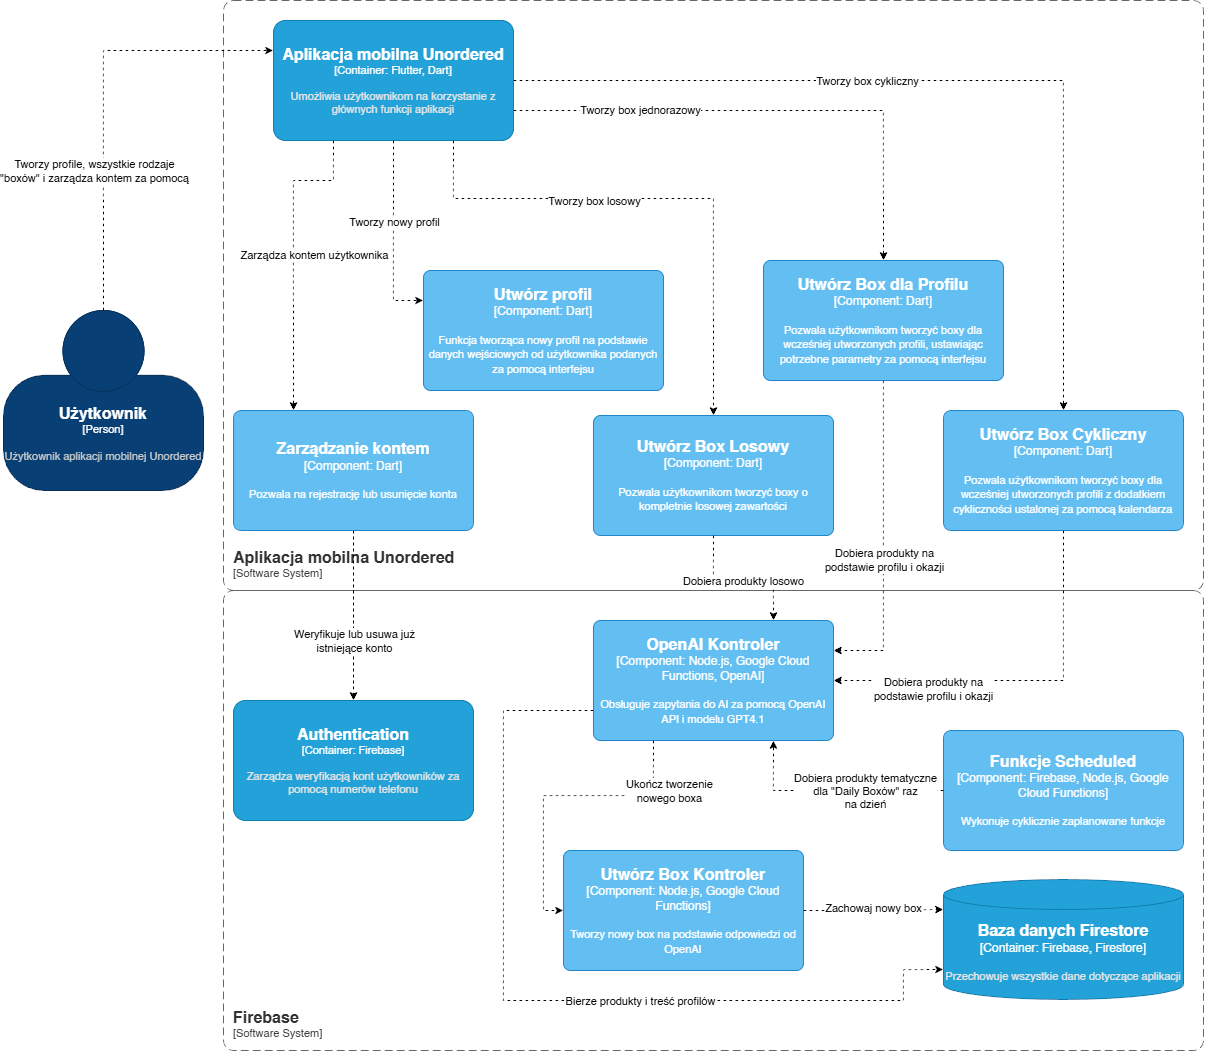
\includegraphics[width=.8\textwidth]{images/unordered.c4.png}
    \caption{Architektura systemu}{Źródło: drawio.com}
    \label{fig:arch}
\end{figure}

\newpage

\subsection{Frontend (Flutter)}
\todo{Opis frontendu fluttera i wgl}
\begin{itemize}
    \item Wersja Flutter: [X.Y.Z]
    \item Główne pakiety: \texttt{firebase\_core}, \texttt{cloud\_functions}, \texttt{http}, etc.
    \item Struktura katalogów:
    \begin{lstlisting}[language=bash]
    \end{lstlisting}
\end{itemize}

\subsection{Backend (Firebase)}
\begin{itemize}
    \item \textbf{Baza danych:} Firestore - przechowuje dane użytkowników, zapisane profile, utworzone boxy, listy produktów i jakiekolwiek inne potrzebne dane do działania aplikacji.
    \item \textbf{Funkcjonalość:} Cloud Functions (Node.js) - obsługuje główne działania backendu aplikacji, takie jak generowanie boxów, komunikacja i przetwarzanie danych z OpenAI czy pobieranie aktualnej listy produktów.
    \item \textbf{Uwierzytelnianie:} Firebase Authentication - pozwala użytkownikom na rejestrację i logowanie się do aplikacji za pomocą numeru telefonu, używając weryfikacji SMS.
    \item \textbf{Automatyzacja:} Cloud Functions Scheduler - służy do cyklicznego uruchamiania funkcji, obsługuje m.in. generowanie ``Daily Boxów'' - codziennych propozycji prezentów o losowych kategoriach.
\end{itemize}

\newpage
\section{Funkcjonalności}
\todo{Pokazać w screenshotach jak to działa albo to zrobić w sekcji frontend}
\subsection{Generowanie boxów}

\subsubsection{Typy generowania}
\begin{itemize}
    \item \textbf{Dla profilu} - Generacja boxów na podstawie profilu, który został wcześniej utworzony.
    Użytkownik podaje budżet oraz okazję, na którą box ma być wygenerowany.
    \item \textbf{Cykliczny} - Generacja boxów cyklicznych,
    które będą generowane co określony czas (np. co miesiąc, co rok).
    Wymagane parametry jak w przypadku boxów ``Dla profilu''.
    \item \textbf{Losowy} - Generacja losowych propozycji prezentów, bez podawania żadnych parametrów
    \item \textbf{Manualny} - aktualnie brak implementacji
\end{itemize}

\subsubsection{Profil użytkownika}
Do wygenerowania boxów typu ``Dla profilu'' lub ``Cykliczny'' wymagane jest utworzenie profilu, dla którego dobierane będą propozycje. Dane profilu to:
\begin{itemize}
    \item \textbf{Nazwa profilu} (np. ``Mama'', ``Tata'', ``Kolega'')
    \item \textbf{Opis osoby} (Preferencje, zainteresowania, itp.)
    \item \textbf{Zainteresowania} (Wybór kategorii z gotowej listy)
\end{itemize}

\subsection{Struktura boxa}
Struktura boxów jest taka sama dla wszystkich typów generowania. Boxy są przechowywane w bazie danych Firestore i zawierają następujące dane:
\begin{itemize}
    \item \textbf{Budżet} (Kwota, którą użytkownik chce przeznaczyć na prezenty)
    \item \textbf{Data wygenerowania} (Data, kiedy box został wygenerowany)
    \item \textbf{Czy jest cykliczny} (Wartość boolean, czy box jest cykliczny)
    \item \textbf{Frekwencja cykliczności} (Użyte tylko dla boxów cyklicznych, np. co miesiąc, co rok)
    \item \textbf{Okazja} (Okazja, na którą box został wygenerowany, np. urodziny, imieniny)
    \item \textbf{Planowana data} (Data, na którą box został zaplanowany)
    \item \textbf{Cena} (Suma cen wszystkich produktów w boxie)
    \item \textbf{Lista produktów} (Produkty, które zostały wygenerowane w boxie)
\end{itemize}

\section{Integracja z OpenAI}
\subsection{Opis API}
Wybranym do generacji modelem jest \textbf{gpt-o4-mini}.
Wybór modelu jest uzasadniony
jego działaniem w trybie ``reasoning'' który pozwala na generacje biorącą pod
uwagę wszystkie parametry podane przez użytkownika.
Jest on również tańszym wyborem, w porównaniu do modeli \textbf{gpt-4.1} oraz \textbf{gpt-o3}.
\subsection{Prompt engineering}
Przy inżynierii promptów uwaga była skupiona na wykorzystaniu najmniejszej ilości tokenów
przy zachowaniu jak najlepszej jakości odpowiedzi.
Strukturą wszystkich promptów jest:
\textbf{ZASADA}$\rightarrow$\textbf{OPIS ZASADY}
\begin{itemize}
    \item \textbf{Generowanie boxów dla profilu} - generacja boxów na podstawie profilu użytkownika.\\\\
        \textbf{ANALIZA}$\rightarrow$Uwzględnij zainteresowania, okazję (...) \\
        \textbf{RÓŻNORODNOŚĆ}$\rightarrow$Unikaj powtórzeń, (...) \\
        \textbf{BUDŻET}$\rightarrow$Nigdy nie przekraczaj budżetu!(...) \\
        \textbf{ODPOWIEDŹ}$\rightarrow$Zwróć TYLKO JSON array (...) \\
    \item \textbf{Generowanie ``Daily Boxów''} - generacja boxów o różnych tematach, raz dziennie.\\\\
        \textbf{DOBÓR}$\rightarrow$Uwzględnij temat, unikaj innych kategorii. (...) \\
        \textbf{RÓŻNORODNOŚĆ}$\rightarrow$Unikaj powtórzeń,  (...) \\
        \textbf{BUDŻET}$\rightarrow$Nigdy nie przekraczaj budżetu!  (...) \\
        \textbf{ODPOWIEDŹ}$\rightarrow$Zwróć TYLKO JSON array  (...) \\
    \item \textbf{Generowanie losowych boxów} - generacja boxów bez podawania żadnych parametrów.\\\\
        \textbf{LOSOWOŚĆ}$\rightarrow$Wybierz losowe przedmioty (...) \\
        \textbf{RÓŻNORODNOŚĆ}$\rightarrow$Dobieraj różne kategorie. \\
        \textbf{BUDŻET}$\rightarrow$Utrzymaj realistyczny budżet.\\
        \textbf{ODPOWIEDŹ}$\rightarrow$Zwróć TYLKO JSON array (...) \\
\end{itemize}
\subsection{Przetwarzanie odpowiedzi}
Formatem zwróconej odpowiedzi jest JSON array, który zawiera listę samych ID produktów,
aby zminimalizować ilość tokenów. Następnie ID są sprawdzane oraz przetwarzane przez backend.

\section{Wdrożenie}
\subsection{Konfiguracja Firebase}
Aby wdrożyć funkcje chmurowe (Cloud Functions) za pomocą Firebase, należy użyć narzędzia \texttt{firebase} dostępnego przez npm, oraz zainicjować projekt i wdrożyć funkcję do projektu Firebase.
Po wdrożeniu należy upewnić się, że adresy (linki) do nowych funkcji są zgodne zarówno w kodzie backendu (Cloud Functions), jak i w wywołaniach po stronie frontendu Flutter. Spójność nazw i endpointów jest kluczowa dla poprawnej komunikacji między aplikacją a backendem.

\newpage
\section{Podsumowanie i dalszy rozwój}
\todo{Zrobić podsumowanie i rozwój}
\subsection{Znane ograniczenia}
\begin{itemize}
    \item Ograniczenia, limity związane np z OpenAI, firebase, etc.
\end{itemize}

\subsection{Roadmap}
Planowane funkcje (np. integracja z sklepami).

\begin{thebibliography}{9}
\bibitem{flutter}
Flutter documentation, \url{https://flutter.dev/docs}

\bibitem{firebase}
Firebase documentation, \url{https://firebase.google.com/docs}

\bibitem{openai}
OpenAI API reference, \url{https://platform.openai.com/docs/api-reference}
\end{thebibliography}

\end{document}